\section{Séance 2 : \'Etude du régulateur PID}
\subsection{Introduction}
La première séance avait pour but d'identifier le système thermique que nous
devons réguler. L'identification du système a permit un premier ensemble de gains
pour un régulateur de type PID en utilisant la méthode de 
\textbf{Chien - Hrones - Reswick}. Les gains trouvés ne sont en aucun cas un optimum,
mais un bon point de départ pour commencer à les optimiser.\\

Cette séance continue à batir sur ce que nous avons trouvé durant la première séance,
en observant l'influence des gains d'un régulateur PID sur notre système. 
Nous alons donc faire plusieurs essais en faisant varier les gains et en comparant
les réponses du sytème régulé, afin de pouvoir visualiser et tirer des conclusions
sur les effets des différents gains du régulateur PID.
 

\subsection{Théorie}

Avant de commencer, nous allons aborder quelque notions théoriques
qui permettront de mieux comprendre le régulateur PID et ainsi
pouvoir tirer des conclusions plus pertinentes de nos essais.

\begin{figure}[H]	
    \centering
    
    \tikzstyle{block} = [draw, fill=blue!20, rectangle, minimum height=3em, minimum width=6em]
    \tikzstyle{sum} = [draw, fill=blue!20, circle, node distance=1cm]
    \tikzstyle{input} = [coordinate]
    \tikzstyle{output} = [coordinate]
    \tikzstyle{tmp} = [coordinate]
    \tikzstyle{pinstyle} = [pin edge={to-,thin,black}]

    \begin{tikzpicture}[auto, node distance=2cm,>=latex']
        % Blocks
        \node [input, name=input] {};
        \node [sum, right of=input] (sum) {};
        \node [block, right of=sum] (controller) {$R(s)$};
        \node [block, right of=controller, node distance=3cm] (system) {$H(s)$};
        \node [output, right of=system] (output) {};

        % Basic Flow
        \draw [->] (input) -- node {$y_{sp}$} (sum);
        \draw [->] (sum) -- node {$\epsilon(s)$} (controller);
        \draw [->] (controller) -- node[name=u] {$u$} (system);
        \draw [->] (system) -- node [name=y] {$y_{pv}$}(output);
        
        % feedback arrow
        \node [tmp, below of=u] (feedback_tmp) {};
        \draw [->] (y) |- (feedback_tmp) -| node[pos=0.99] {$-$} (sum);

        %\node (input) [left of=system,node distance=2cm, coordinate] {system};
        %\node [coordinate] (output) [right of=system, node distance=2cm]{};
        %\path[->] (input) edge node {$i$} (system);
        %\path[->] (system) edge node {$T^\circ$} (output);
    \end{tikzpicture}
    \caption{Schéma bloc du système avec régulateur}
\end{figure}

\subsubsection{Régulateur P}
Le régulateur P (proportionnel) est le cas le plus simple.
La commande de sortie est uniquement définie par la différence 
$\epsilon(t)$ entre la valeur désirée, qu'on appelle le \textbf{setpoint}, et
la valeur réelle mesurée, amplifiée par un certain gain $k_p$.

$$u(t) = k_p \cdot \epsilon(t)$$

Le problème de ce régulateur est que si la valeur de sortie est
égale au setpoint ou s'en approche, la commande sera nulle ou
presque. Dans le cas de nôtre système thermique, si la température
mesurée approche la température désirée, le courant à travers la
résistance sera nulle. Du à la déperdition thermique, la température
chutera et on ne pourra donc pas maintenir le setpoint.\\

Pour palier à se problème, nous pouvons ajouter un offset à la 
commande qui permet de contrer exactement la déperdition:

$$u(t) = k_p \cdot \epsilon(t) + U_0$$

Cependant, la déperdition thermique, et donc cet offset, dépendent 
de la différence de température entre le système et l'air ambiant.
Si on change le setpoint il faut un offset différent. 


\subsubsection{Régulateur PI}
Le régulateur PI (proportionnel - intégrale), est déjà nettement plus pratique
puisqu'il permet d'obtenir cet l'offset variable sans trop d'efforts. Le terme intégrale va augmenter 
tant que l'erreur est positive. Une fois que l'erreur est nulle, 
le terme intégrale reste constant. 

$$u(t) = k_p \left( \epsilon(t) + \frac{1}{T_i} \int \limits_0^t \epsilon(t) \; dt \right)$$

Le terme proportionnel va avoir beaucoup d'influence
au début, quand l'erreur est grande. Il permet donc de donner du punch au début.
Mais au fur et a mesure que l'erreur diminue, son influence diminue également.
C'est alors que le terme intégrale joue son rôle, comme il intègre l'erreur
il va grandir tant qu'un erreur est présente. On va donc progressivement
s'approcher de la valeur désirée et une fois qu'on la atteinte, se terme
reste constant.

Cependant, il faut faire attention à ne pas trop abuser du terme intégrale.
Si son coefficient est trop grand, on va créer des problèmes de dépassement
(\textit{'overshoot'}) et d'oscillations, voir même rendre le système instable.

\subsubsection{Régulateur PID}
Finalement, dans le régulateur PID (proportionnel - intégrale - dérivée), on 
ajoute un terme dérivée:

$$u(t) = k_p \left( \epsilon(t) + \frac{1}{T_i} \int \limits_0^t \epsilon(t) \; dt + T_d \frac{d\epsilon(t)}{dt} \right)$$

Ce terme permet de réduire les oscillations en s'opposant aux variations
brusques de l'erreur. Il faut par contre le doser avec grand soin, car ce
terme peut grandement amplifier le bruit du système si son coefficient est
trop grand. 

\subsection{Essais}
A la suite de la première séance, nous avons trouvés les valeurs de gains suivants
à l'aide de la méthode de Chien - Hrones - Reswick:

\begin{center}
    $K_0  = 4.118$
    \hspace{1cm}
    $T_{i0} = 145.830$
    \hspace{1cm}
    $T_{d0} = 15.662$
    \hspace{1cm}
    $T_{f0} = 1.041$
\end{center}

\paragraph{\textcolor{red}{Note:}}\mbox{}\\
A la suite de la première mesure, qui a durée très longtemps par rapport aux autres groupes,
nous avions l'impression que notre gain proportionnel $K_0$ que nous avions trouvé à l'aide de la méthode de 
Chien - Hrones - Reswick était relativement faible, du à l'imprécision sur la détermination graphique 
de $T_{U}$ et $T_{G}$. Durant le premier essai, décrit dans la section \ref{essai-0}, nous avons constaté que 
le système mettait énormément de temps à se stabiliser, soit approximativement 9 minutes. Suivi d'encore 10 minutes
pour chaque perturbation. Nous avons donc pensé qu'en augmentant le coefficient proportionnel pour le
reste des manipulations, nous pourrions diminuer le temps nécessaire à chaque mesurer et ainsi terminer les 9 essais dans les temps.
Ceci à été fait en conecertation avec l'enseignant, bien entendu.\\

Soit si on indique le gain trouvé initialement par $K_0'$, nous avons décidé de 
prendre comme gain durant le reste des mesures 

$$K_0 = 1.5 \cdot K_0' = 6.177$$

Il s'est avéré plus tard, dans la section sur l'optimisation du régulateur \ref{opt-reg}, que ce n'était pas
le coefficient proportionnel qui était trop faible, mais le terme intégratif qui avait trop peu d'influence.


\pagebreak
\subsubsection{Essai 0 : $K_{p} = 0.66*K_{0}'$, $T_{i} = T_{i0}$ et $T_{d} = T_{d0}$} \label{essai-0}
% Correspond aux mesures matlab s2e0
Comme mentionné dans le paragraphe précédent, le premier essai s'est fait avec
la valeur initiale $K_0'$ trouvée par la méthode de Chien - Hrones - Reswick.
Cependant comme nous avons corrigé le gain de base $K_0$ après cette essai, nous
retiendrons cette essai, avec $K = 0.66 \cdot K_0$, comme l'essai qu'il fallait
faire avec un gain $K = 0.5 \cdot K_0$.

\begin{figure}[H]
    \centering
    % Line 1
    \makebox[\textwidth][c]{
        \begin{subfigure}[b]{0.37\textwidth}
            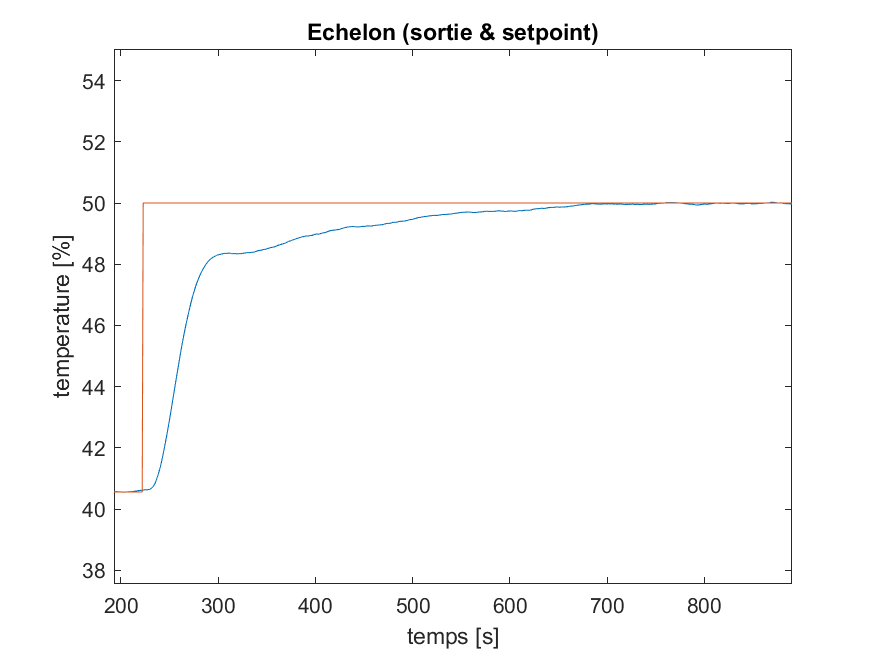
\includegraphics[width=\textwidth]{essais/s2e0-step-out}
        \end{subfigure}
        ~
        \begin{subfigure}[b]{0.37\textwidth}
            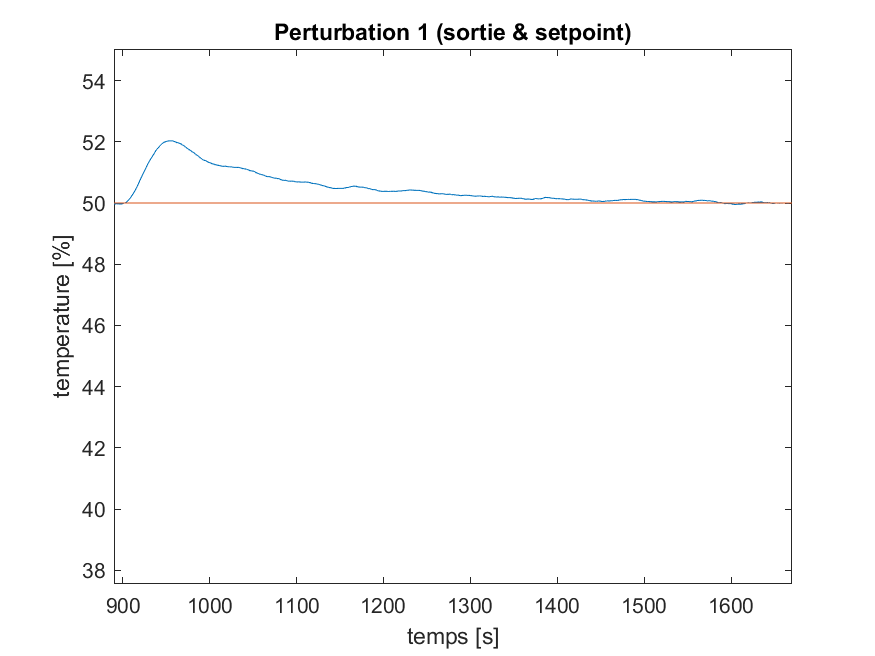
\includegraphics[width=\textwidth]{essais/s2e0-pert-up-out}
        \end{subfigure}
        ~
        \begin{subfigure}[b]{0.37\textwidth}
            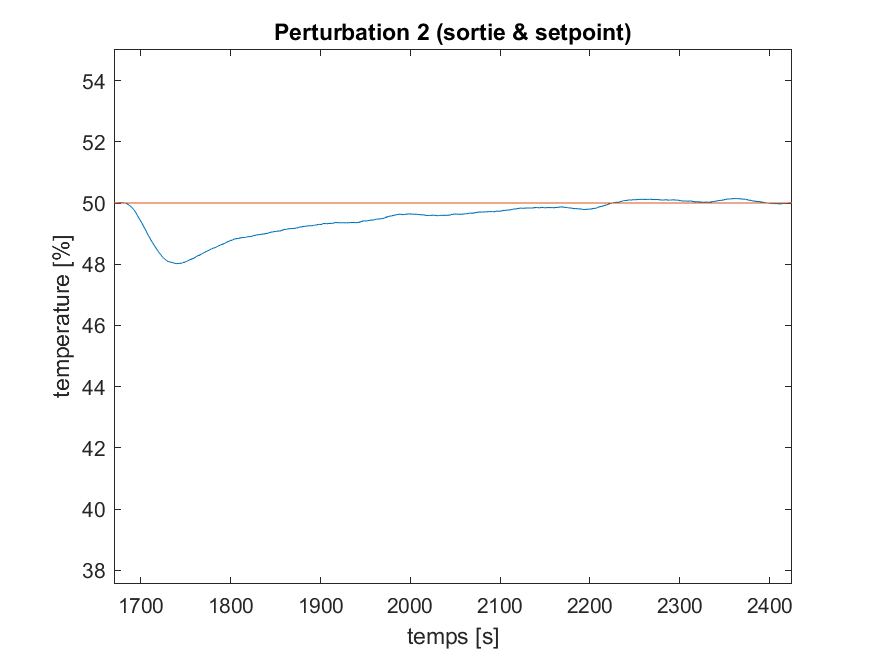
\includegraphics[width=\textwidth]{essais/s2e0-pert-down-out}
        \end{subfigure}
    }
    % Line 2
    \makebox[\textwidth][c]{
        \begin{subfigure}[b]{0.37\textwidth}
            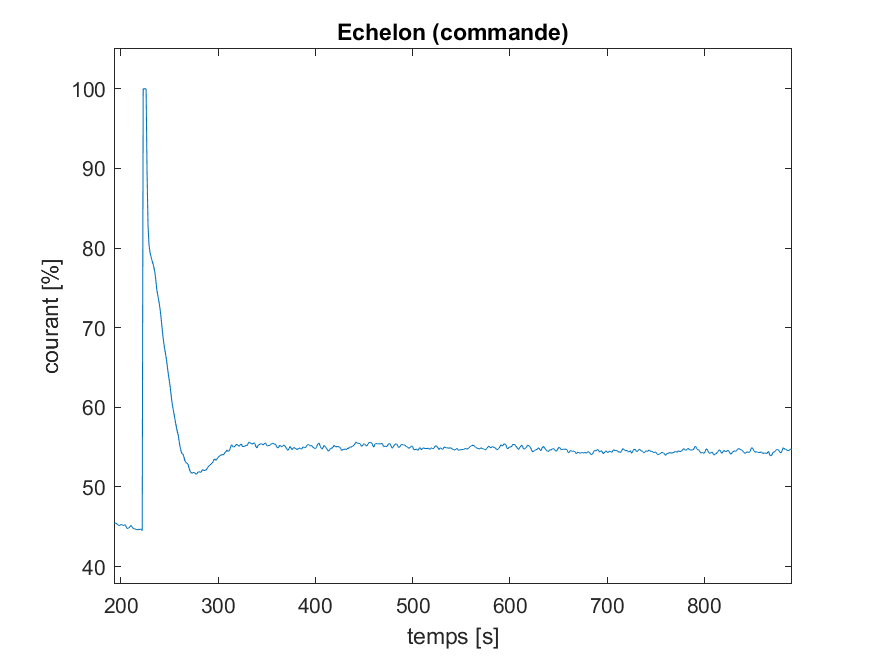
\includegraphics[width=\textwidth]{essais/s2e0-step-command}
        \end{subfigure}
        ~
        \begin{subfigure}[b]{0.37\textwidth}
            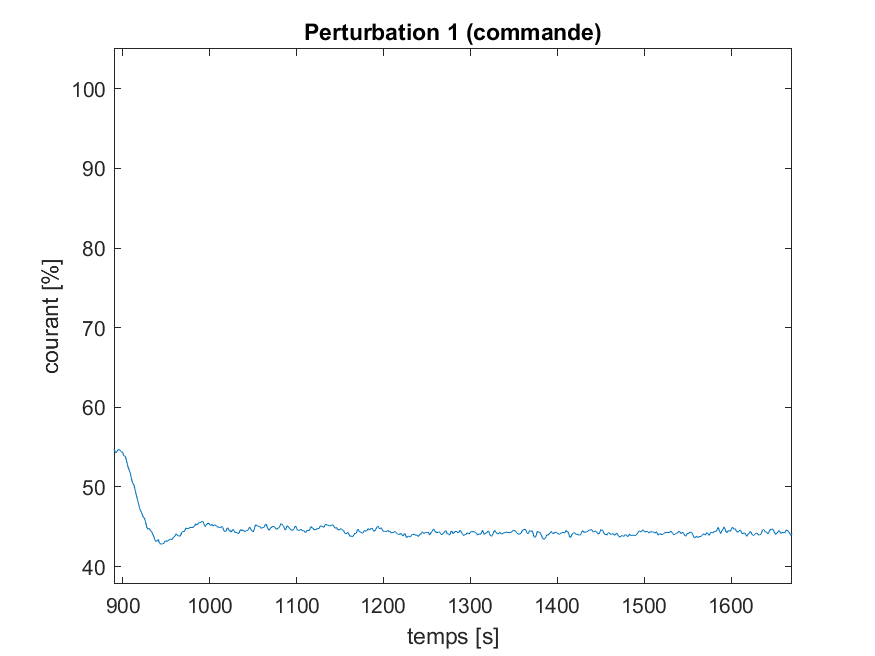
\includegraphics[width=\textwidth]{essais/s2e0-pert-up-command}
        \end{subfigure}
        ~
        \begin{subfigure}[b]{0.37\textwidth}
            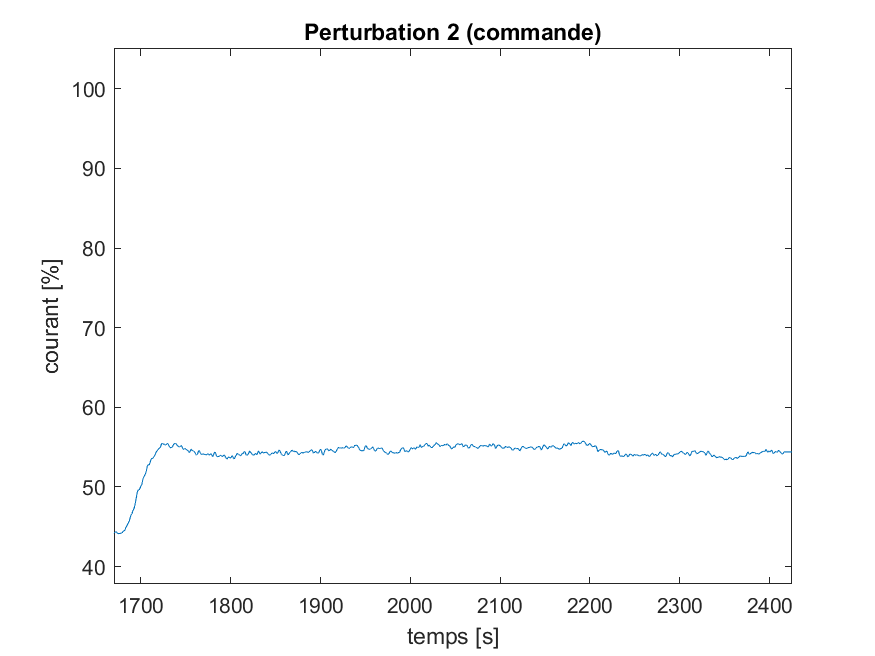
\includegraphics[width=\textwidth]{essais/s2e0-pert-down-command}
        \end{subfigure}
    }
    \caption{Graphes essai 0}
    \label{fig:essai-0}
\end{figure}

Dans cet essais, suite à l'échelon, on peut voir que le système prend un peu 
plus de 8 min à se stabiliser. Dans la première minute, on peut clairement
observer l'action du terme proportionnel. Comme l'erreur est grande, 
il va générer une action importante, ce qui est représenté par le pic
dans le graphe de la commande.\\

Ensuite, comme l'erreur diminue rapidement, le terme proportionnel diminue également.
Et la on peut voir l'effet du terme intégratif qui va progressivement venir
diminuer l'erreur statique jusqu'à être stable au setpoint.

\paragraph{\textcolor{red}{Note:}}\mbox{}\\
Les diagrammes de Bodes que nous avons générés sont étranges avec des valeurs de gain et 
phases énormes. Nous en avons discuté brièvement avec M. Arnould, mais n'avons pas reussi à
déterminer l'origine de ces grandes valeurs. Nous mettrons donc les diagrammes de bodes que
nous avons calculés dans le rapport, mais notterons qu'aucune interprétation n'en a été faite,
de peur de tirer de mauvaises conclusions. 

\fig{essais/bode-0}{0.5}{Diagramme de Bode}

\subsubsection{Essai 1 : $K_{p} = K_{0}'$, $T_{i} = T_{i0}$ et $T_{d} = T_{d0}$}
%Correspond au fichier s2e1 

\begin{figure}[H]
    \centering
    % Line 1
    \makebox[\textwidth][c]{
        \begin{subfigure}[b]{0.37\textwidth}
            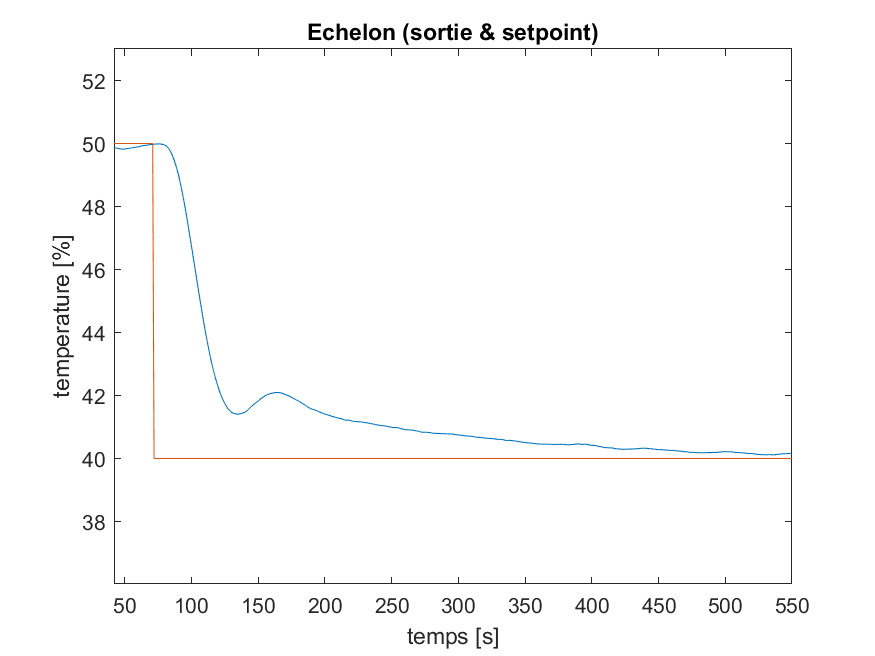
\includegraphics[width=\textwidth]{essais/s2e1-step-out}
        \end{subfigure}
        ~
        \begin{subfigure}[b]{0.37\textwidth}
            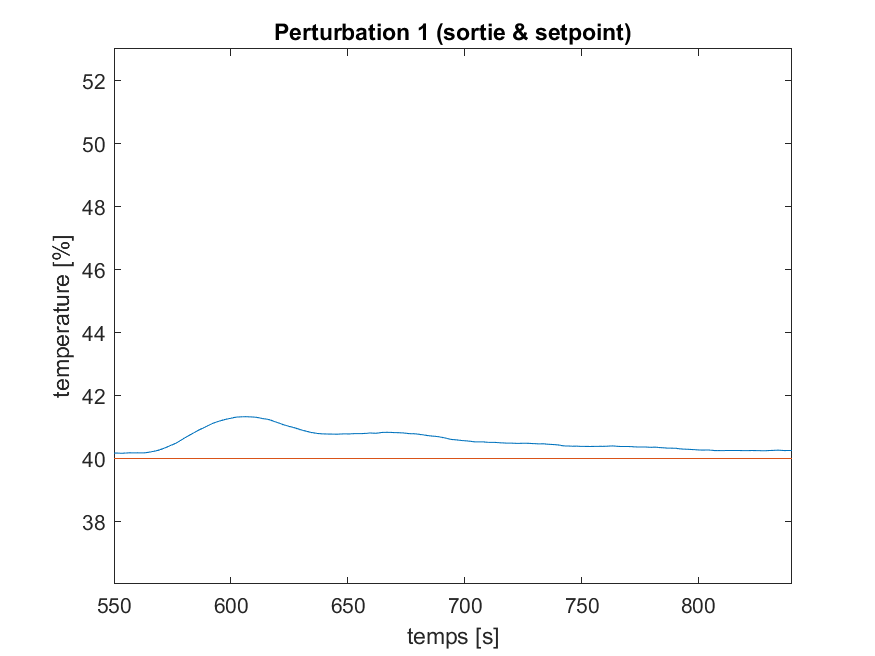
\includegraphics[width=\textwidth]{essais/s2e1-pert-up-out}
        \end{subfigure}
        ~
        \begin{subfigure}[b]{0.37\textwidth}
            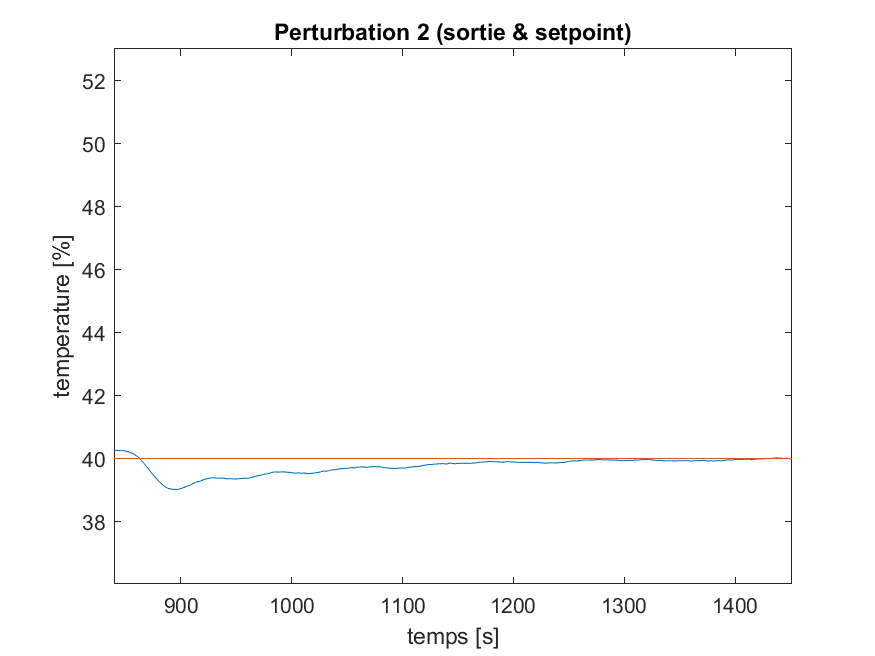
\includegraphics[width=\textwidth]{essais/s2e1-pert-down-out}
        \end{subfigure}
    }
    % Line 2
    \makebox[\textwidth][c]{
        \begin{subfigure}[b]{0.37\textwidth}
            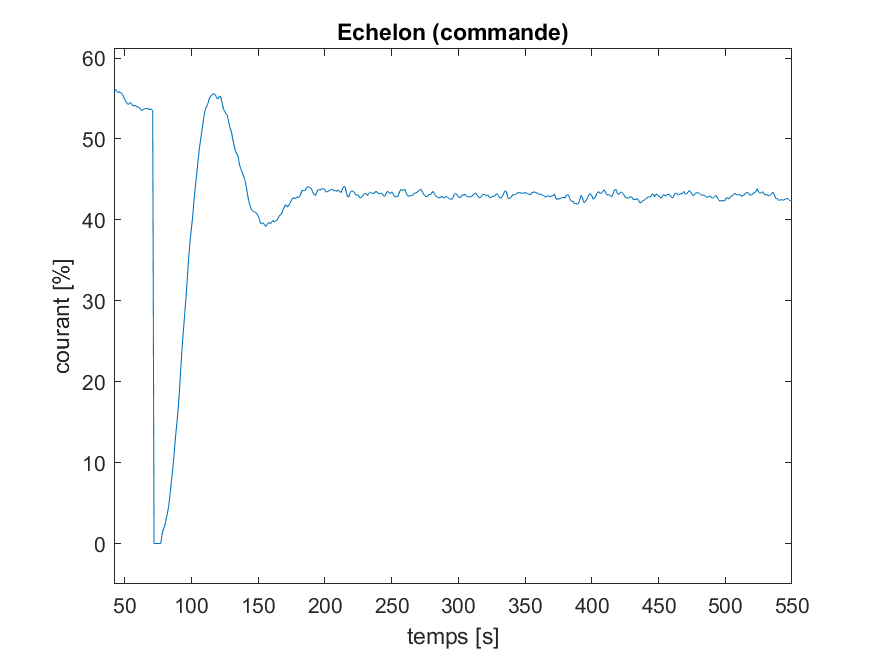
\includegraphics[width=\textwidth]{essais/s2e1-step-command}
        \end{subfigure}
        ~
        \begin{subfigure}[b]{0.37\textwidth}
            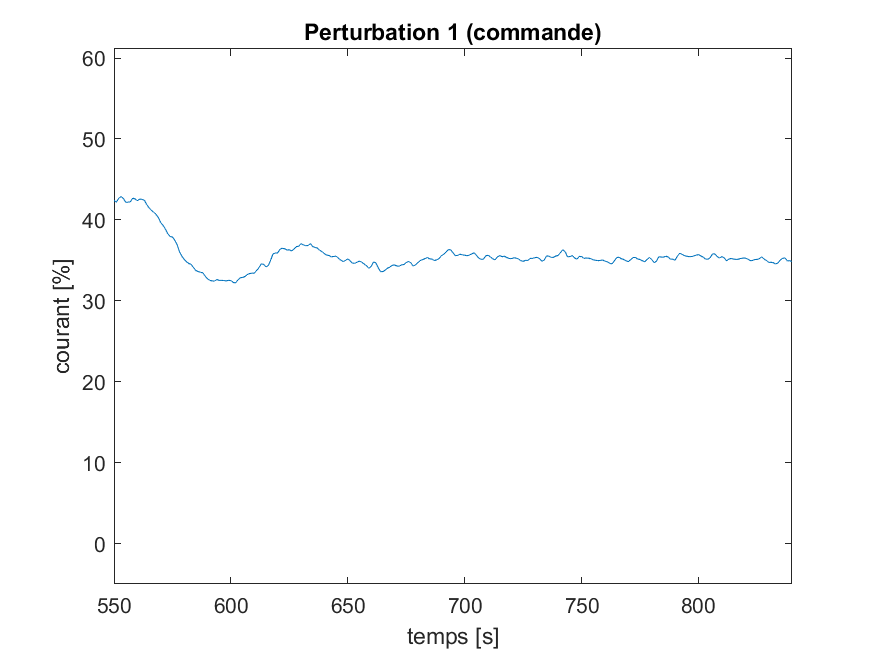
\includegraphics[width=\textwidth]{essais/s2e1-pert-up-command}
        \end{subfigure}
        ~
        \begin{subfigure}[b]{0.37\textwidth}
            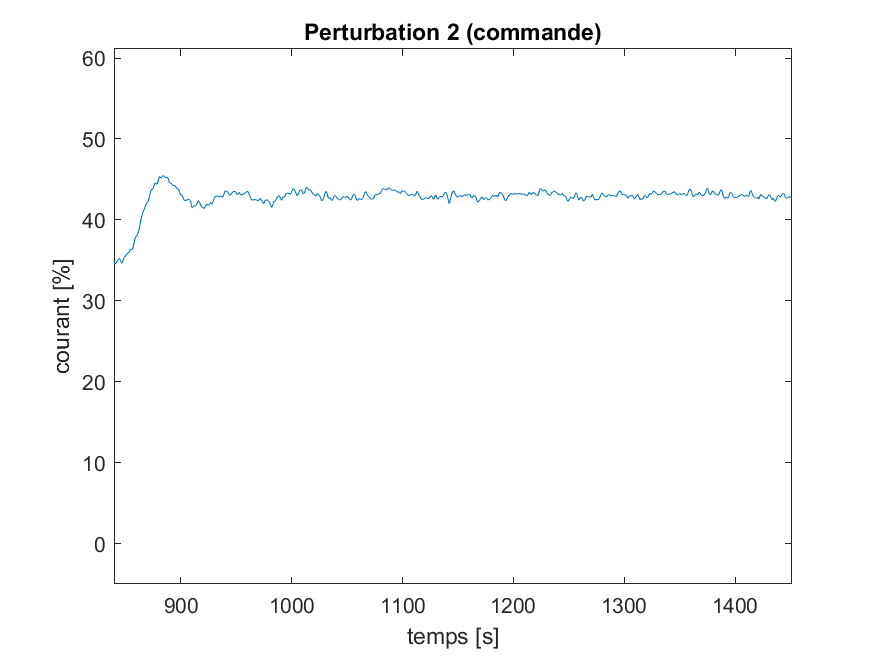
\includegraphics[width=\textwidth]{essais/s2e1-pert-down-command}
        \end{subfigure}
    }
    \caption{Graphes essai 1}
    \label{fig:essai-1}
\end{figure}

Dans cet essai, on peut voir que l'augmentation du terme proportionnel introduit
une légère oscillation avant que le système se stabilise.

\fig{essais/bode-1}{0.5}{Diagramme de Bode}

\subsubsection{Essai 2 : $K_{p} = 0.5*K_{0}'$, $T_{i} = T_{i0}$ et $T_{d} = T_{d0}$}
L'essai 2 n'as pas été fait, comme nous avons pris le premier essai \ref{essai-0}
qui le remplace.

\subsubsection{Essai 3 : $K_{p} = K_{0}'$, $T_{i} = 10^{5}$ et $T_{d} = T_{d0}$}
%Correspond au fichier s2e3
% \begin{figure}[H]
%     \centering
%     % Line 1
%     \makebox[\textwidth][c]{
%         \begin{subfigure}[b]{0.37\textwidth}
%             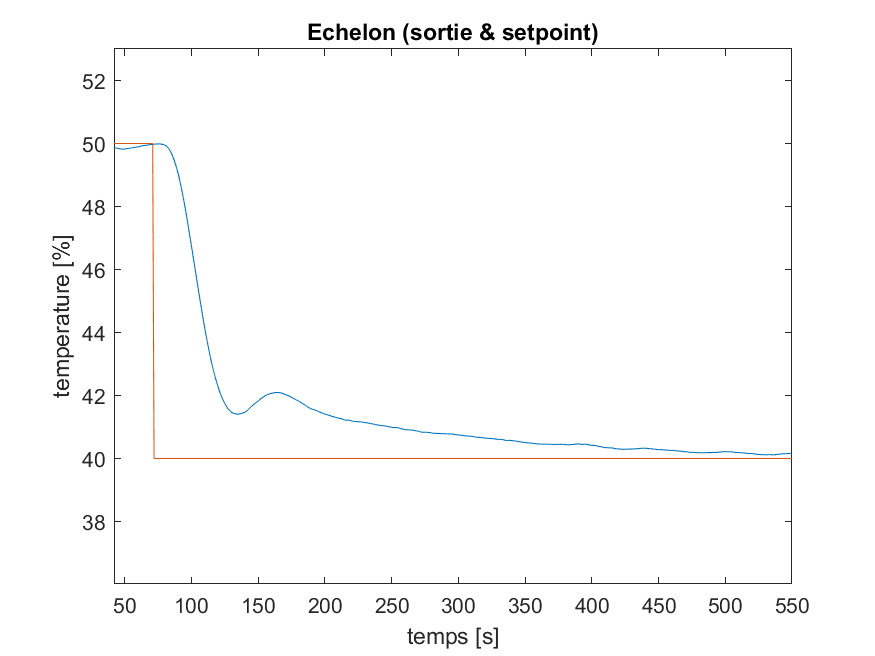
\includegraphics[width=\textwidth]{essais/s2e3-step-out}
%         \end{subfigure}
%         ~
%         \begin{subfigure}[b]{0.37\textwidth}
%             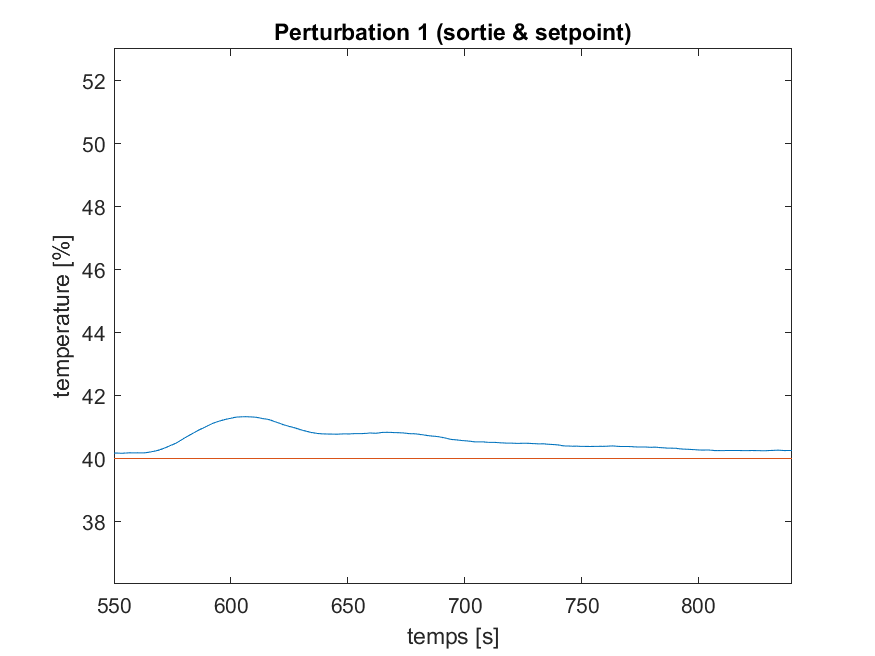
\includegraphics[width=\textwidth]{essais/s2e3-pert-up-out}
%         \end{subfigure}
%         ~
%         \begin{subfigure}[b]{0.37\textwidth}
%             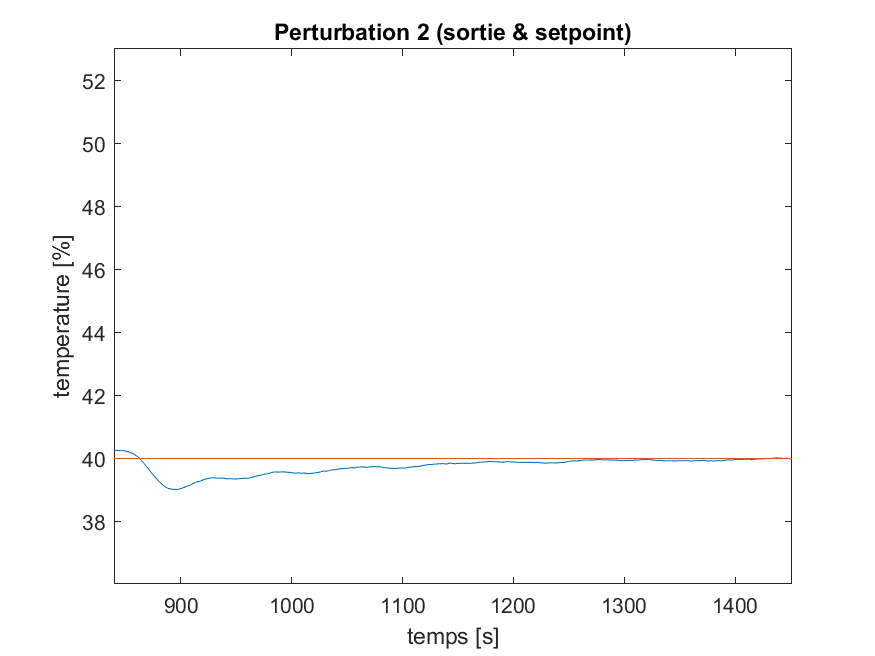
\includegraphics[width=\textwidth]{essais/s2e3-pert-down-out}
%         \end{subfigure}
%     }
%     % Line 2
%     \makebox[\textwidth][c]{
%         \begin{subfigure}[b]{0.37\textwidth}
%             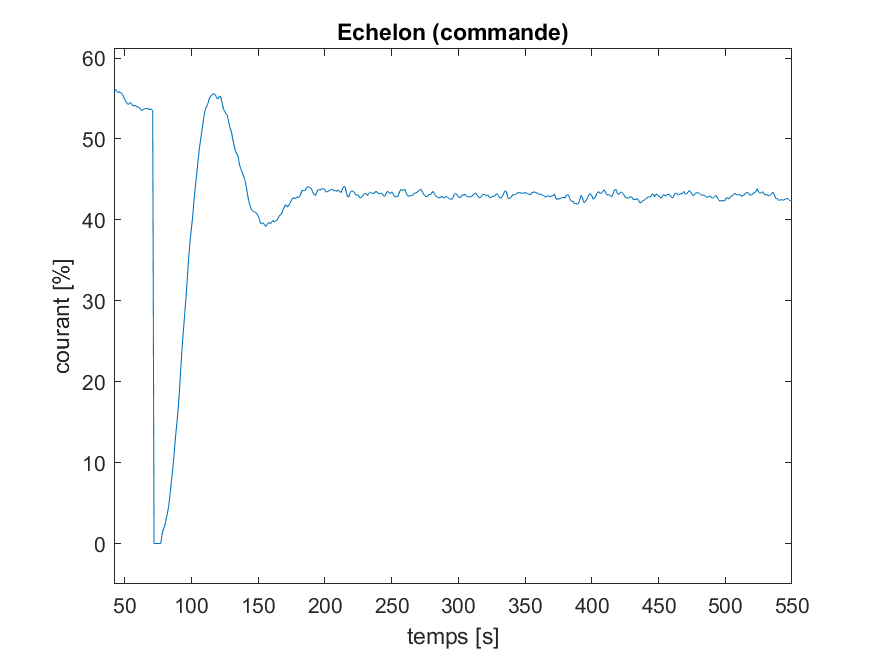
\includegraphics[width=\textwidth]{essais/s2e3-step-command}
%         \end{subfigure}
%         ~
%         \begin{subfigure}[b]{0.37\textwidth}
%             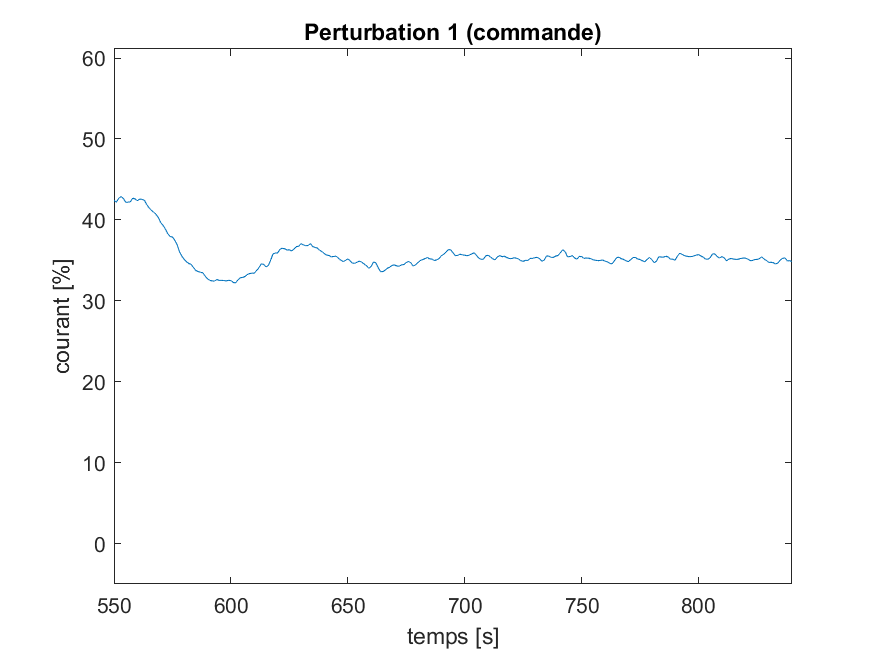
\includegraphics[width=\textwidth]{essais/s2e3-pert-up-command}
%         \end{subfigure}
%         ~
%         \begin{subfigure}[b]{0.37\textwidth}
%             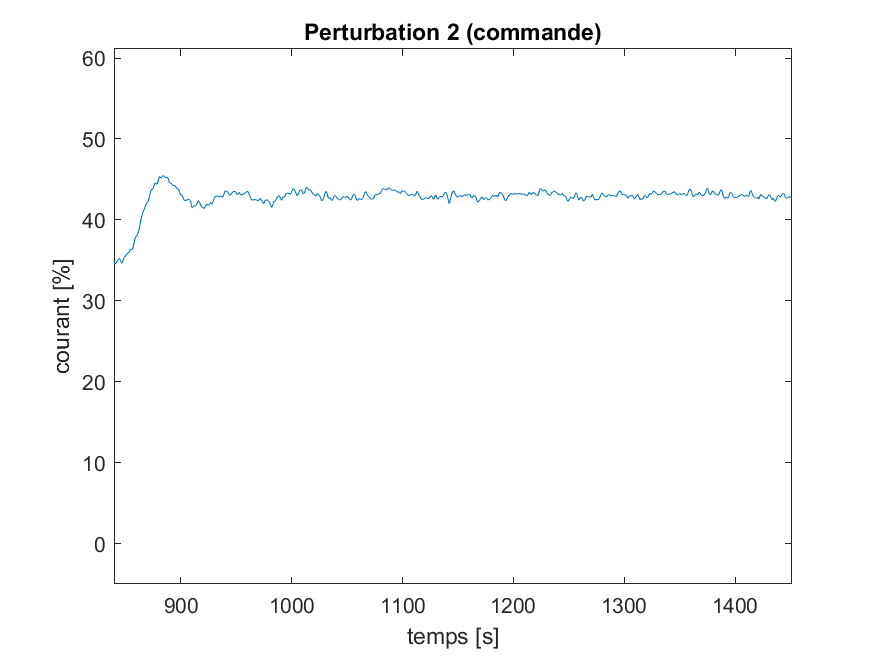
\includegraphics[width=\textwidth]{essais/s2e3-pert-down-command}
%         \end{subfigure}
%     }
%     \caption{Graphes essai 3}
%     \label{fig:essai-3}
% \end{figure}

Dans cet essai, la contribution du terme intégratif est réduit à zéro.\\
Malheureusement, nous avons fait une fausse manipulation et les données de
cet essais n'ont pas été correctement enregistrées...


%\fig{essais/bode-3}{0.5}{Diagramme de Bode}

\subsubsection{Essai 4 : $K_{p} = K_{0}'$, $T_{i} = 10^{5}$ et $T_{d} = 10^{-3}$}
%Correspond au fichier s2e4

\begin{figure}[H]
    \centering
    % Line 1
    \makebox[\textwidth][c]{
        \begin{subfigure}[b]{0.37\textwidth}
            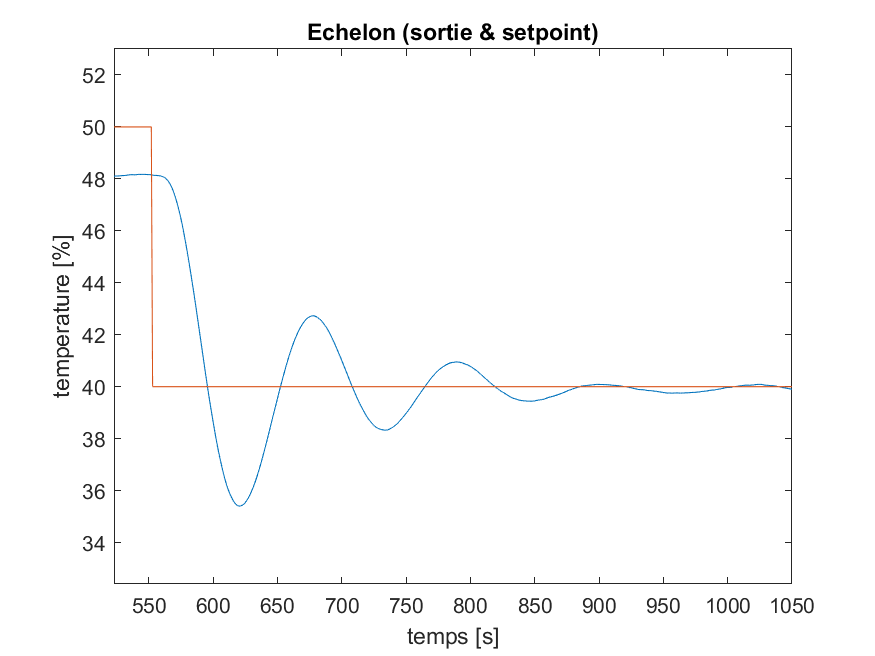
\includegraphics[width=\textwidth]{essais/s2e4-step-out}
        \end{subfigure}
        ~
        \begin{subfigure}[b]{0.37\textwidth}
            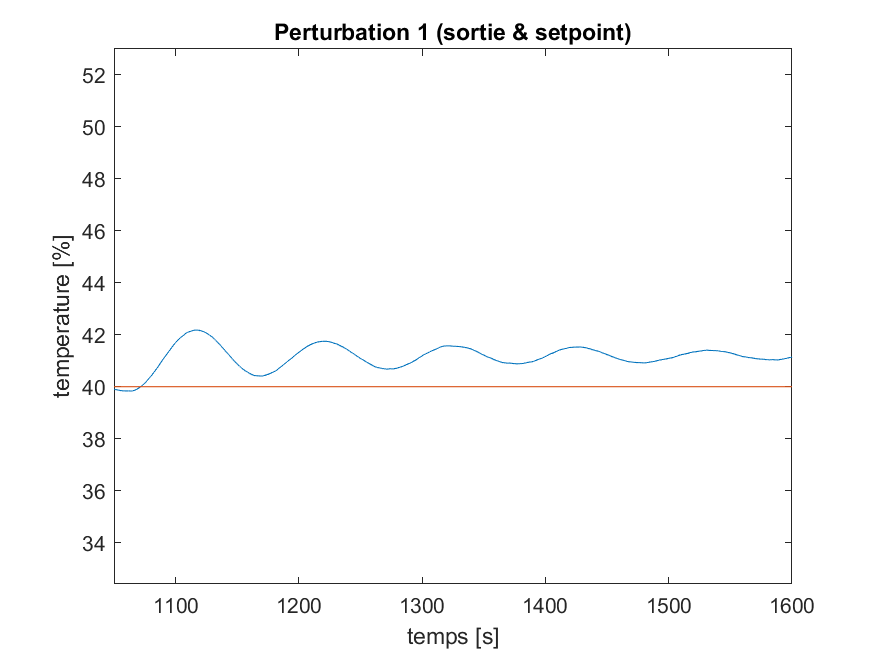
\includegraphics[width=\textwidth]{essais/s2e4-pert-up-out}
        \end{subfigure}
        ~
        \begin{subfigure}[b]{0.37\textwidth}
            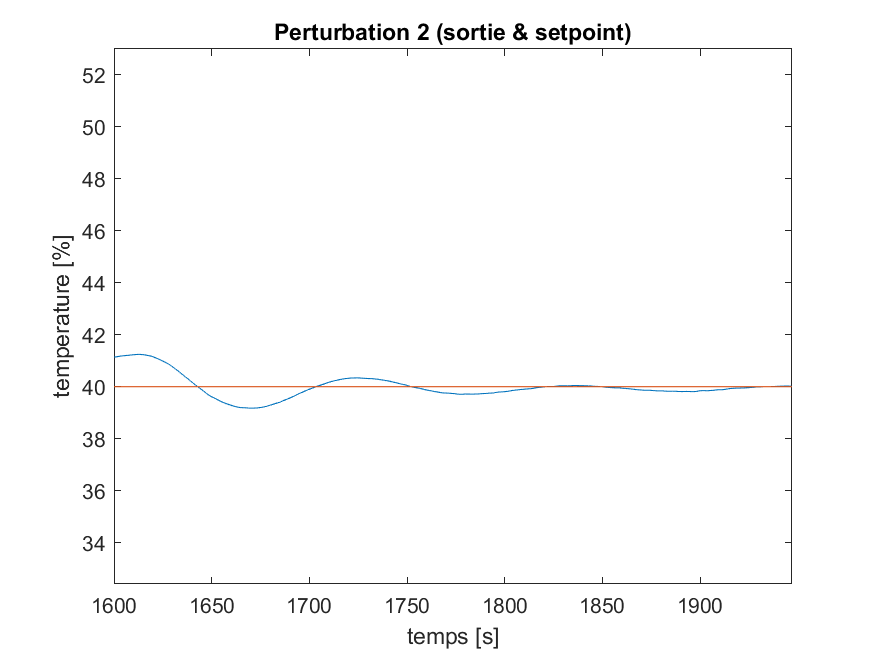
\includegraphics[width=\textwidth]{essais/s2e4-pert-down-out}
        \end{subfigure}
    }
    % Line 2
    \makebox[\textwidth][c]{
        \begin{subfigure}[b]{0.37\textwidth}
            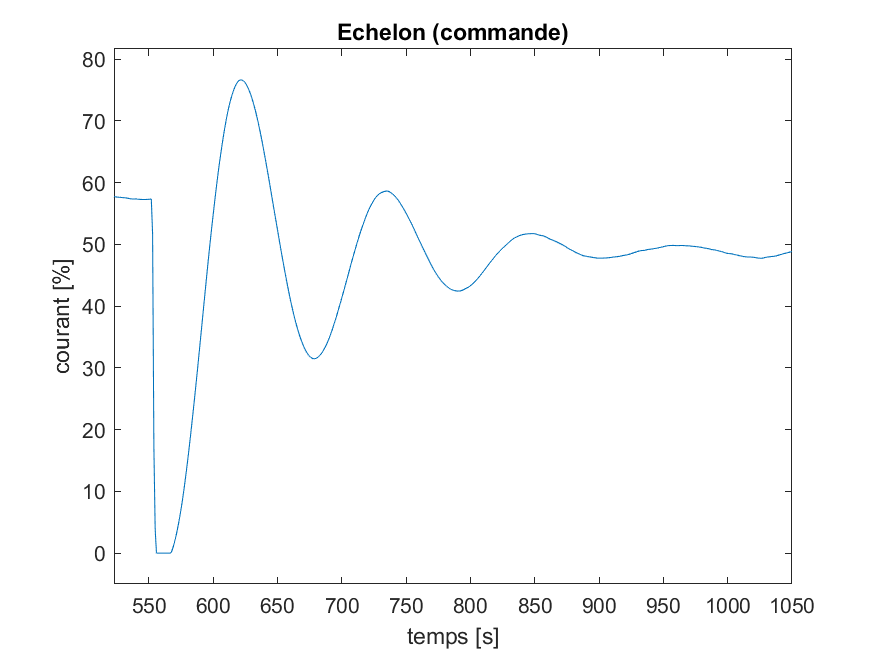
\includegraphics[width=\textwidth]{essais/s2e4-step-command}
        \end{subfigure}
        ~
        \begin{subfigure}[b]{0.37\textwidth}
            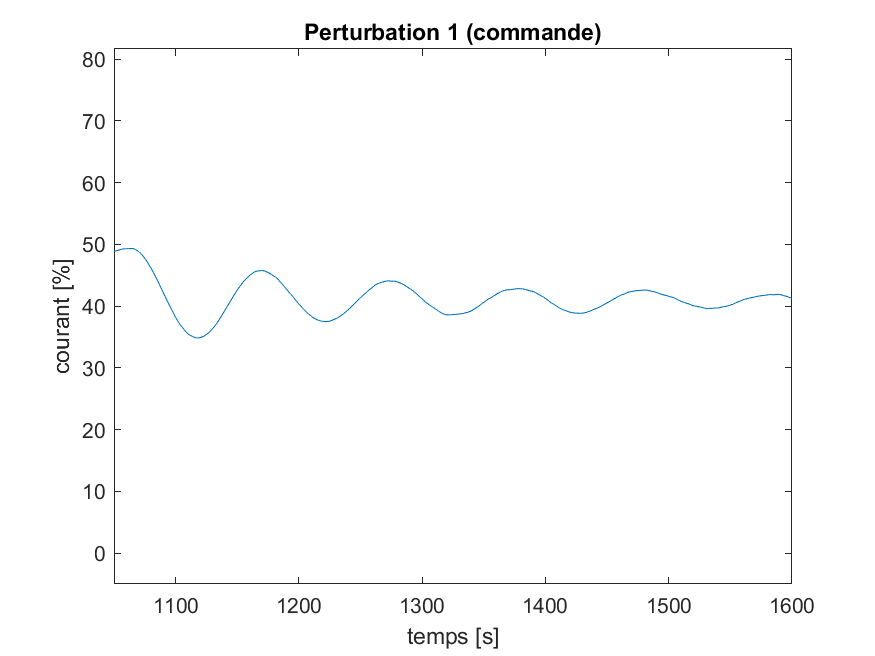
\includegraphics[width=\textwidth]{essais/s2e4-pert-up-command}
        \end{subfigure}
        ~
        \begin{subfigure}[b]{0.37\textwidth}
            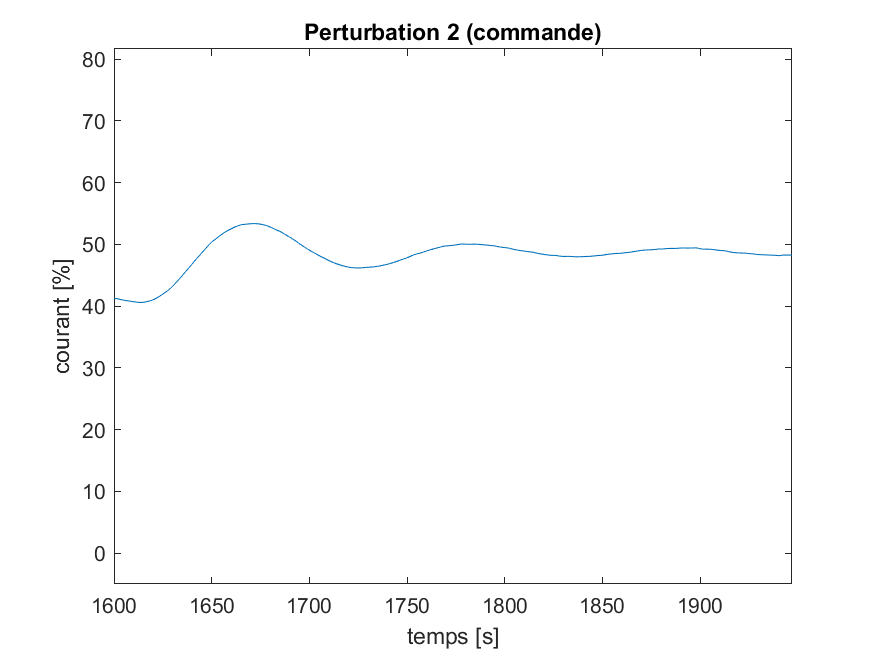
\includegraphics[width=\textwidth]{essais/s2e4-pert-down-command}
        \end{subfigure}
    }
    \caption{Graphes essai 4}
    \label{fig:essai-4}
\end{figure}

Dans l'essai numéro 4, le terme intégratif et dérivatif n'ont pas d'apports.
On a donc un régulateur P, purement proportionnel. On peut voir que pour 
l'échelon, malgré l'oscillation importante, le système a réussi à se stabiliser
sur la valeur du setpoint. Mais quand on regarde le graphe de la première perturbation,
bien que les oscillations diminue, une erreur statique persiste.

Au niveau de la commande, on peut voir une légère saturation juste après avoir appliqué l'échelon.
Ceci est est à éviter, puisqu'on sort du régime linéaire et notre modélisation n'est alors plus correcte.

\fig{essais/bode-4}{0.5}{Diagramme de Bode}

\subsubsection{Essai 5 : $K_{p} = 0.5*K_{0}'$, $T_{i} = 10^{5}$ et $T_{d} = 10^{-3}$}
%Correspond au fichier s2e5

\begin{figure}[H]
    \centering
    % Line 1
    \makebox[\textwidth][c]{
        \begin{subfigure}[b]{0.37\textwidth}
            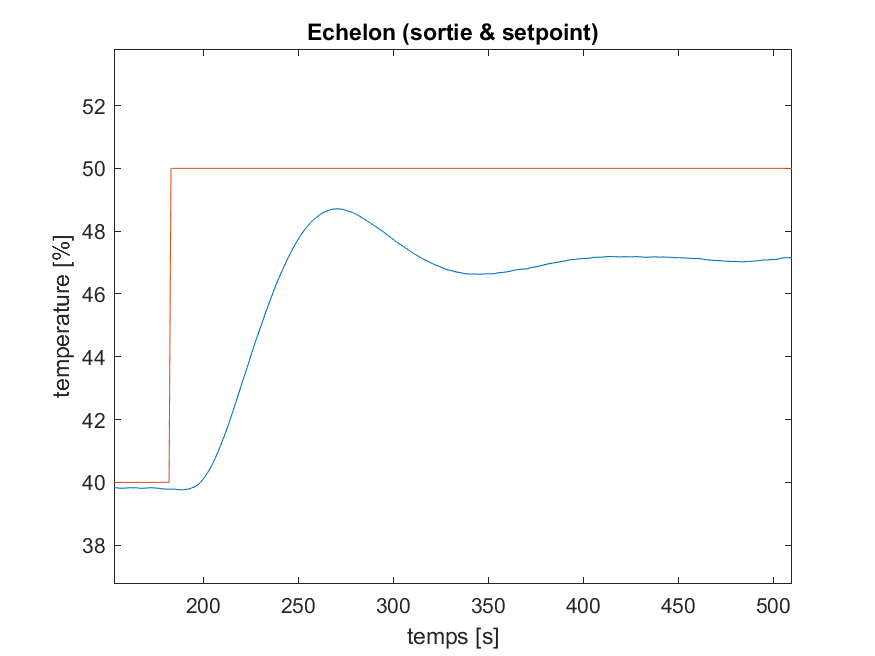
\includegraphics[width=\textwidth]{essais/s2e5-step-out}
        \end{subfigure}
        ~
        \begin{subfigure}[b]{0.37\textwidth}
            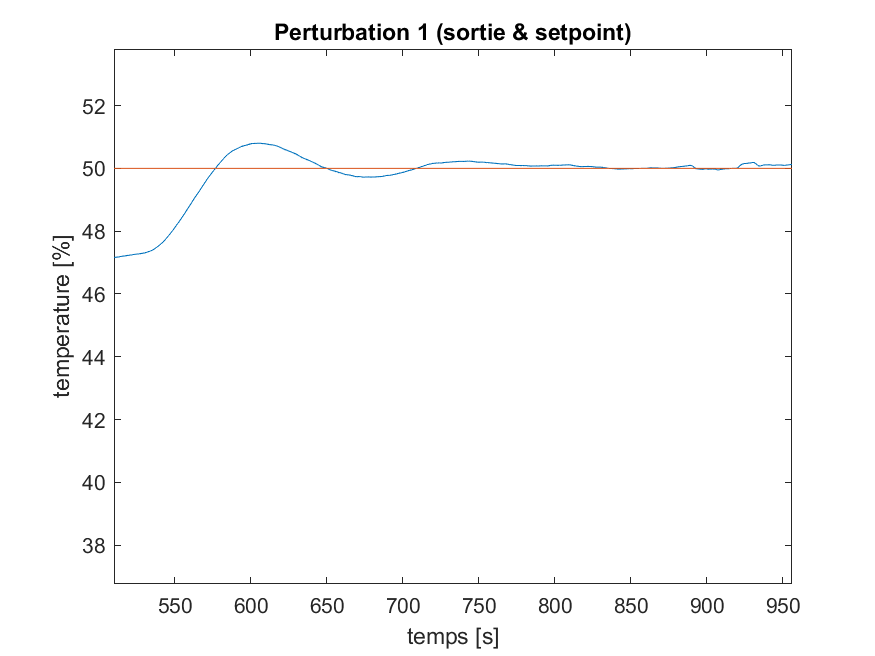
\includegraphics[width=\textwidth]{essais/s2e5-pert-up-out}
        \end{subfigure}
        ~
        \begin{subfigure}[b]{0.37\textwidth}
            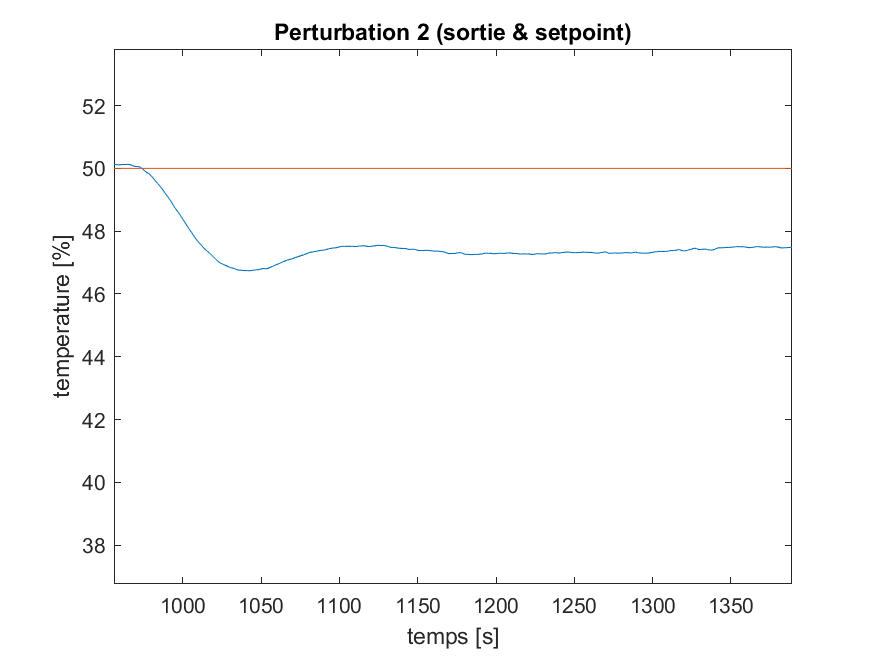
\includegraphics[width=\textwidth]{essais/s2e5-pert-down-out}
        \end{subfigure}
    }
    % Line 2
    \makebox[\textwidth][c]{
        \begin{subfigure}[b]{0.37\textwidth}
            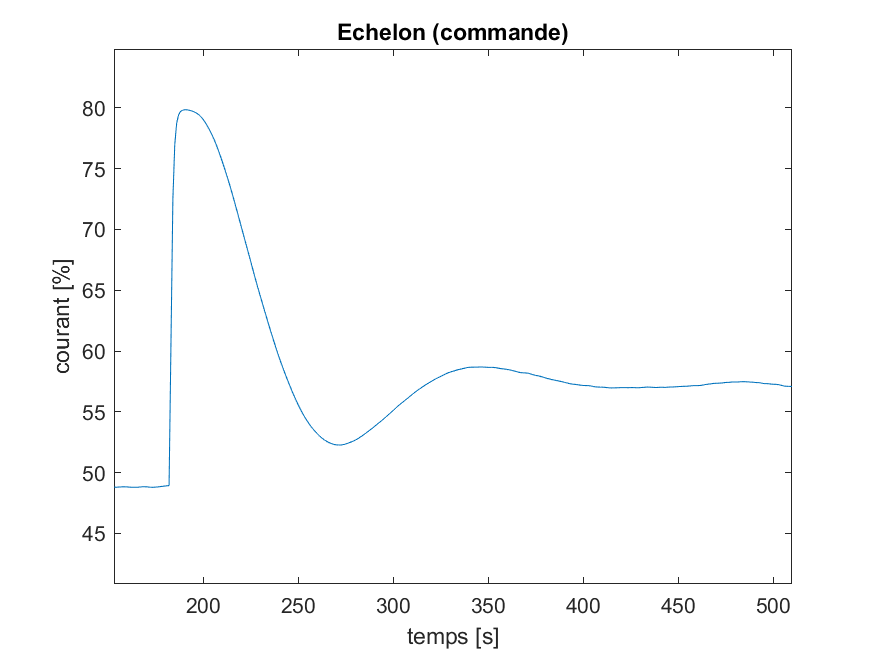
\includegraphics[width=\textwidth]{essais/s2e5-step-command}
        \end{subfigure}
        ~
        \begin{subfigure}[b]{0.37\textwidth}
            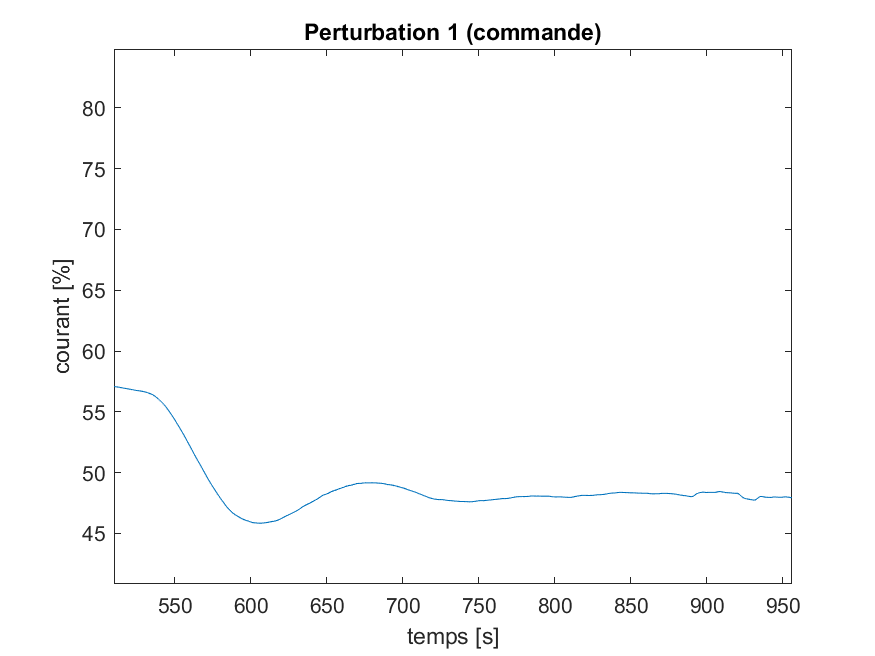
\includegraphics[width=\textwidth]{essais/s2e5-pert-up-command}
        \end{subfigure}
        ~
        \begin{subfigure}[b]{0.37\textwidth}
            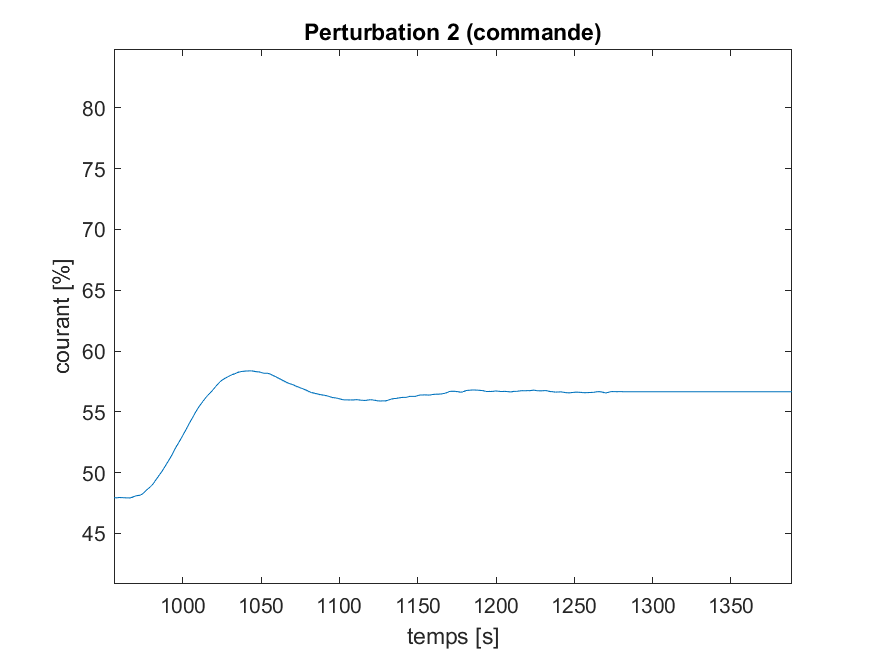
\includegraphics[width=\textwidth]{essais/s2e5-pert-down-command}
        \end{subfigure}
    }
    \caption{Graphes essai 5}
    \label{fig:essai-5}
\end{figure}

Avec la diminution du terme proportionnel, toujours avec les termes intégratif et dérivatif
ayant aucune contribution, on réduit considérablement les oscillations. Mais
comme on peut le voir, l'erreur statique est grande. A la première perturbation,
le système se stabilise à la valeur désirée. Mais comme pour l'essai précédent,
ceci est plus un coup de chance qu'autre chose. Quand la perturbation est à nouveau
supprimée, on peut voir que l'erreur statique est à nouveau présente.

De plus, comparé à l'essai précédent, nous pouvons voir que la commande ne part plus en saturation.
Nous avons même de la marge, puisque nous sommes à 80\%, et pourrions donc le réaugmenter un peu plus.

\fig{essais/bode-5}{0.5}{Diagramme de Bode}

\subsubsection{Essai 6 : $K_{p} = K_{0}'$, $T_{i} = T_{i0}$ et $T_{d} = 2*T_{d0}$}
%Correspond au fichier s2e6


\begin{figure}[H]
    \centering
    % Line 1
    \makebox[\textwidth][c]{
        \begin{subfigure}[b]{0.37\textwidth}
            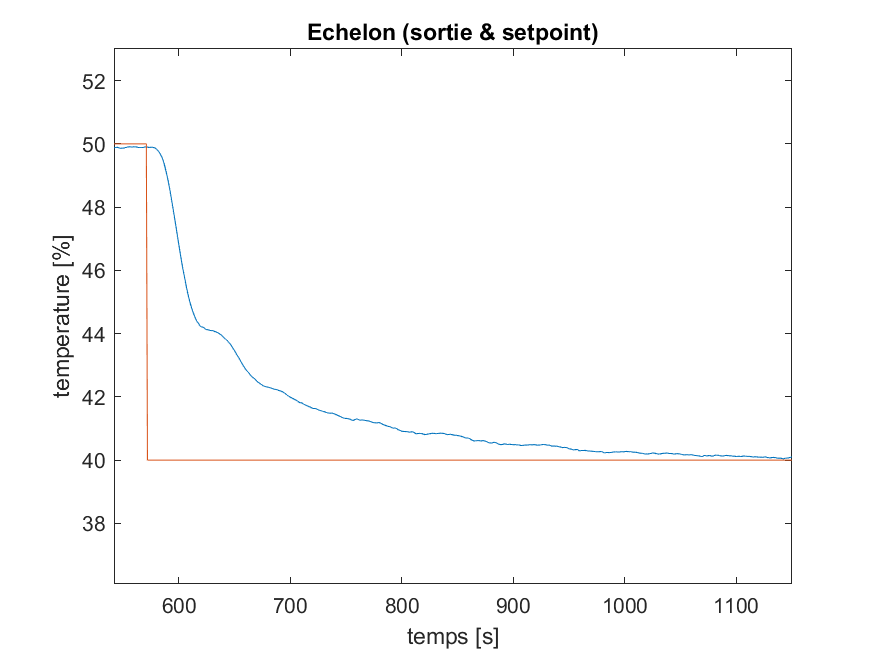
\includegraphics[width=\textwidth]{essais/s2e6-step-out}
        \end{subfigure}
        ~
        \begin{subfigure}[b]{0.37\textwidth}
            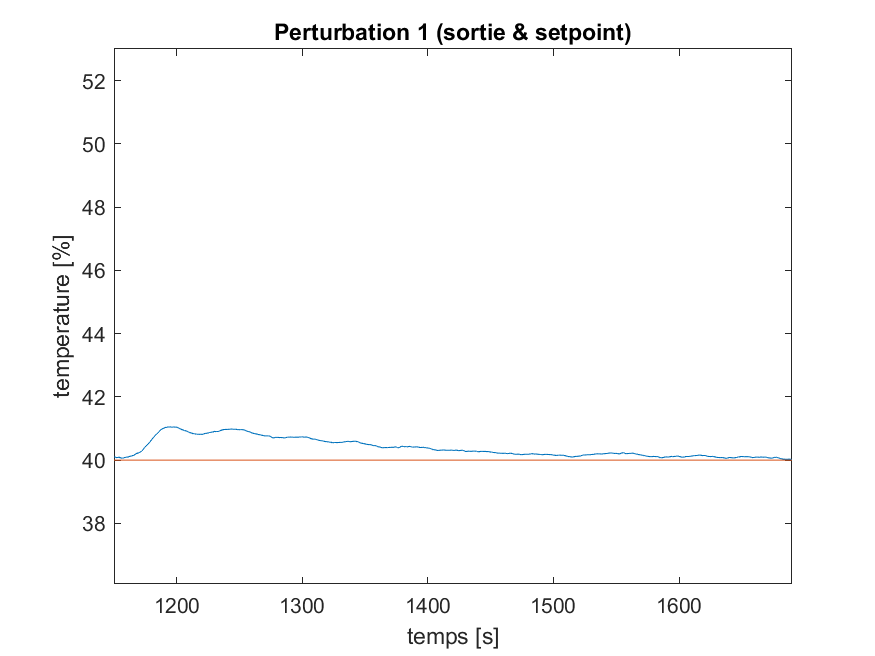
\includegraphics[width=\textwidth]{essais/s2e6-pert-up-out}
        \end{subfigure}
        ~
        \begin{subfigure}[b]{0.37\textwidth}
            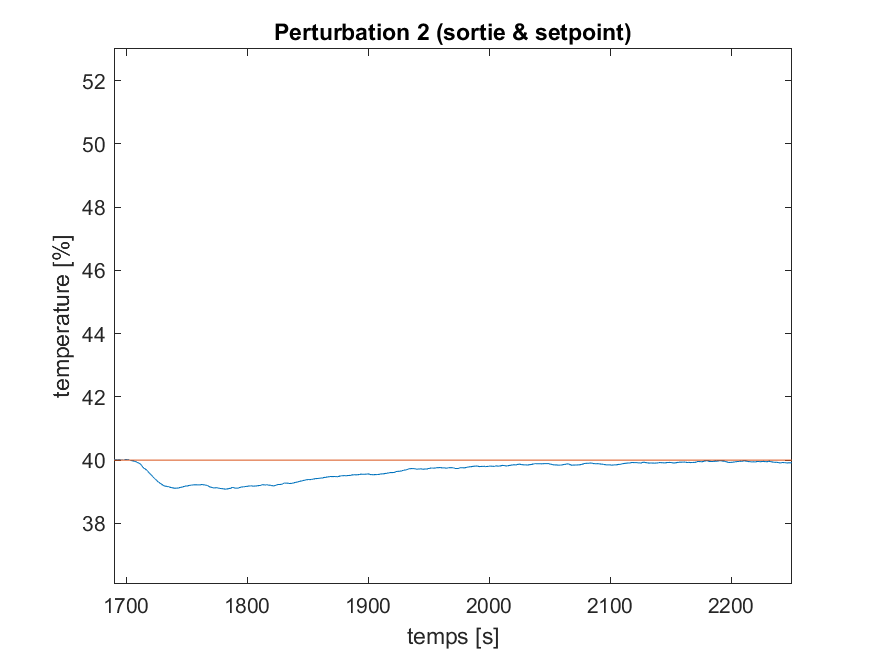
\includegraphics[width=\textwidth]{essais/s2e6-pert-down-out}
        \end{subfigure}
    }
    % Line 2
    \makebox[\textwidth][c]{
        \begin{subfigure}[b]{0.37\textwidth}
            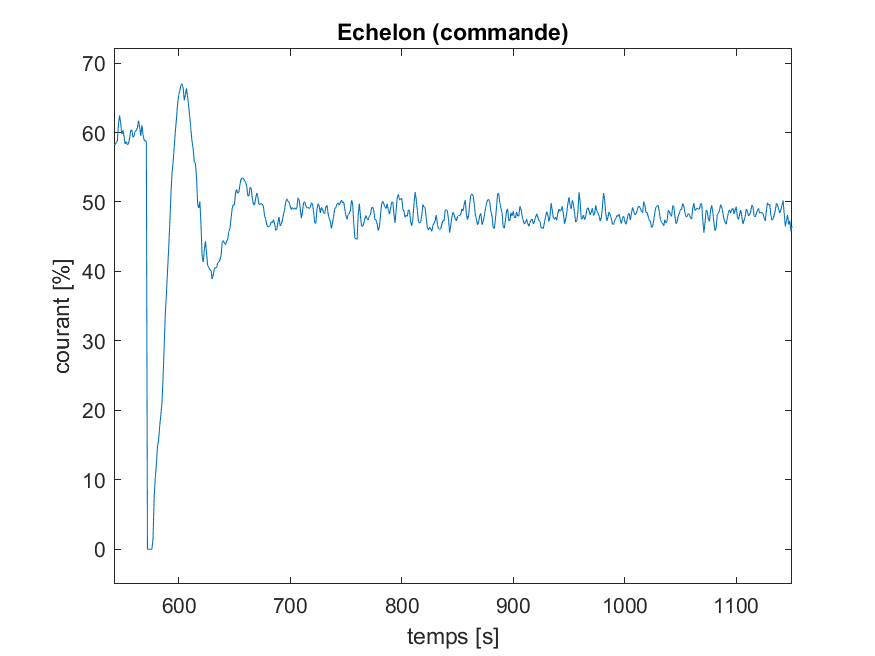
\includegraphics[width=\textwidth]{essais/s2e6-step-command}
        \end{subfigure}
        ~
        \begin{subfigure}[b]{0.37\textwidth}
            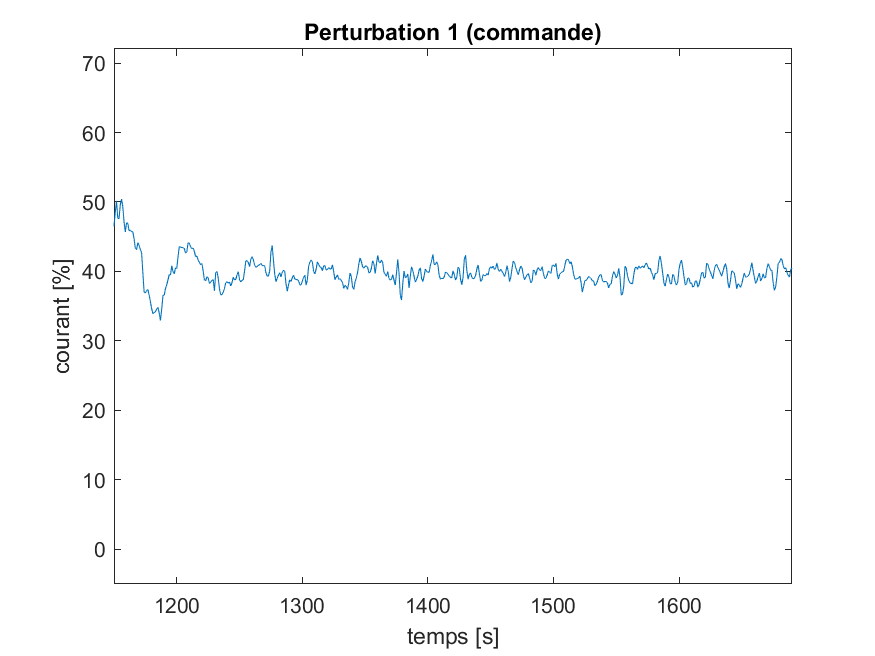
\includegraphics[width=\textwidth]{essais/s2e6-pert-up-command}
        \end{subfigure}
        ~
        \begin{subfigure}[b]{0.37\textwidth}
            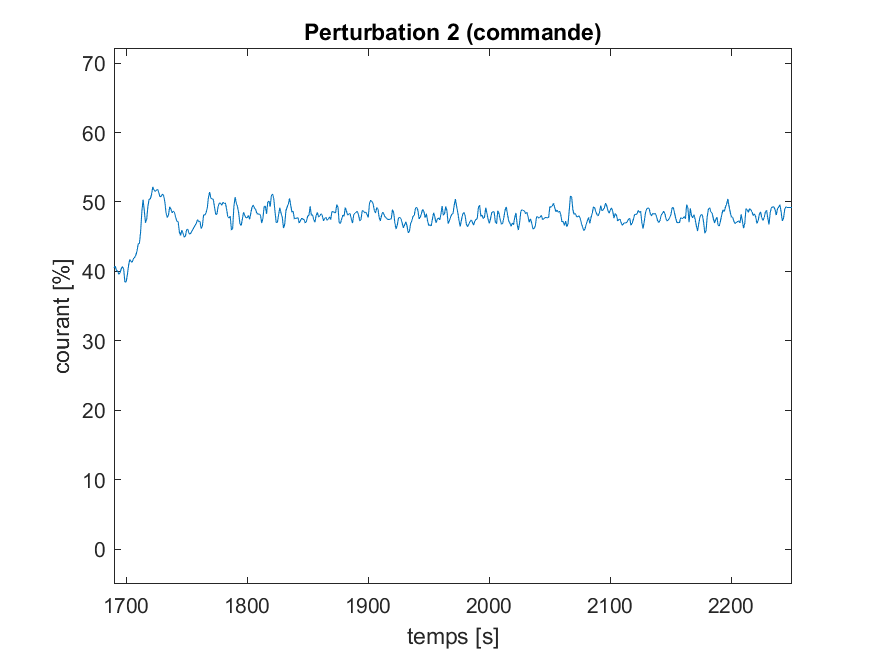
\includegraphics[width=\textwidth]{essais/s2e6-pert-down-command}
        \end{subfigure}
    }
    \caption{Graphes essai 6}
    \label{fig:essai-6}
\end{figure}

En augmentant l'apport du terme dérivatif, on peut remarquer que la commande
est considérablement plus bruitée. Par contre, on peut apercevoir un effet 
bénéfique dans la réaction au perturbations, où la courbe est plus aplatie.

Par contre, nous pouvons voir que l'effet proprotionnel qui donne le coup de punch au début est
également diminué du au terme dérivatif ce qui fait que nous approchones le setpoint de façon plus
lente et progressive.

\fig{essais/bode-6}{0.5}{Diagramme de Bode}

\subsubsection{Essai 7 : $K_{p} = K_{0}$, $T_{i} = T_{i0}$ et $T_{d} = 4*T_{d0}$}
%Correspond au fichier s2e7

\begin{figure}[H]
    \centering
    % Line 1
    \makebox[\textwidth][c]{
        \begin{subfigure}[b]{0.37\textwidth}
            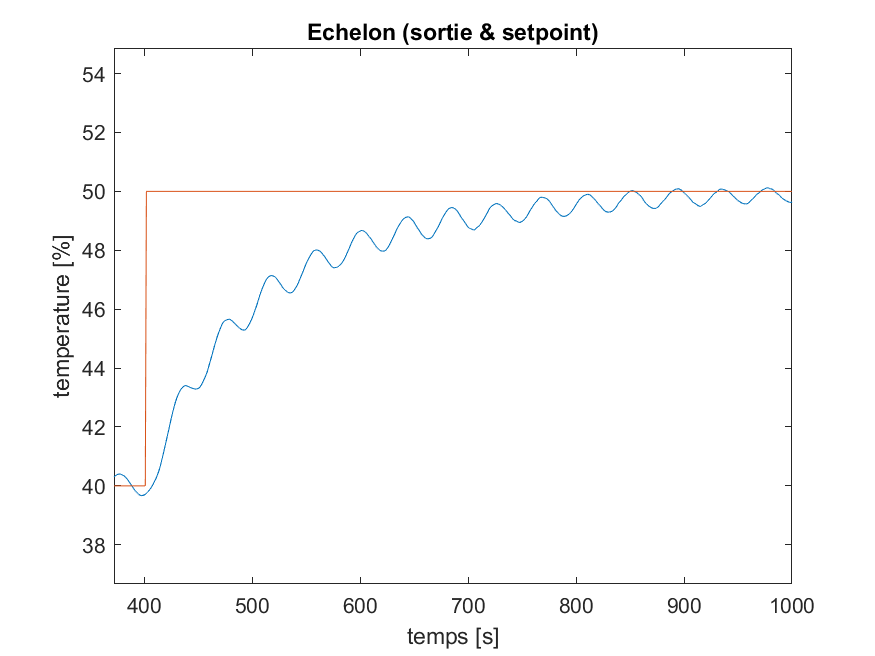
\includegraphics[width=\textwidth]{essais/s2e7-step-out}
        \end{subfigure}
        ~
        \begin{subfigure}[b]{0.37\textwidth}
            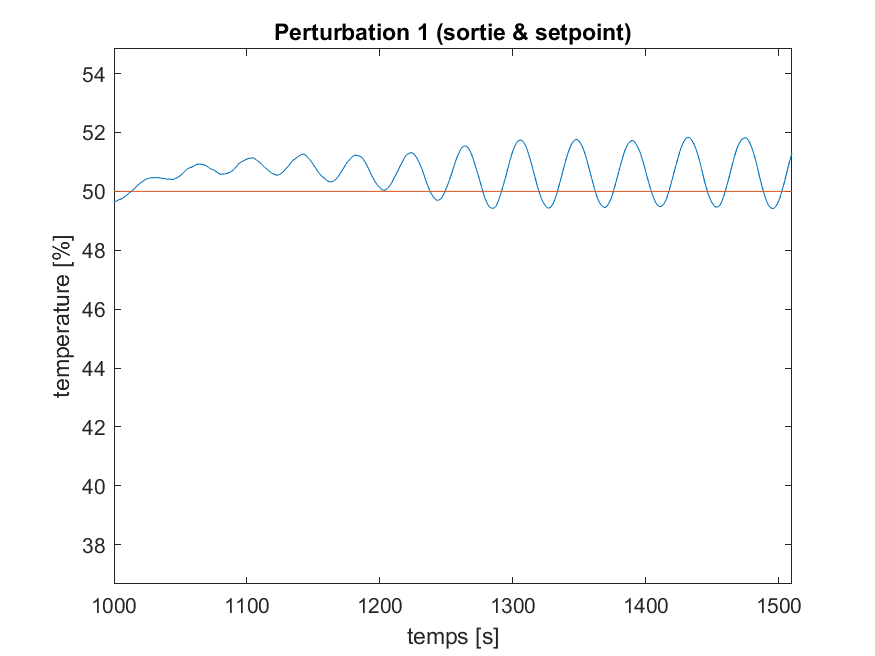
\includegraphics[width=\textwidth]{essais/s2e7-pert-up-out}
        \end{subfigure}
        ~
        \begin{subfigure}[b]{0.37\textwidth}
            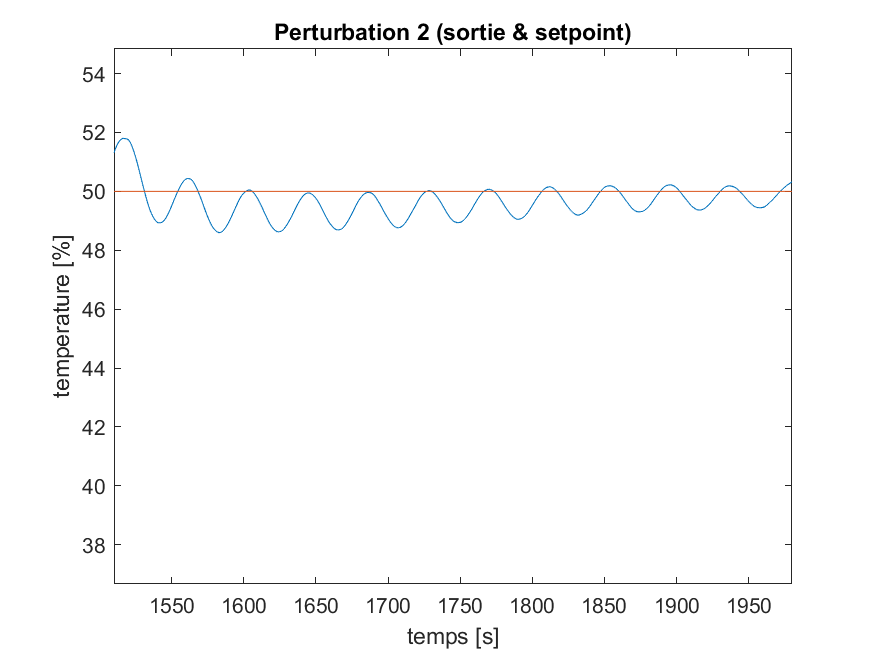
\includegraphics[width=\textwidth]{essais/s2e7-pert-down-out}
        \end{subfigure}
    }
    % Line 2
    \makebox[\textwidth][c]{
        \begin{subfigure}[b]{0.37\textwidth}
            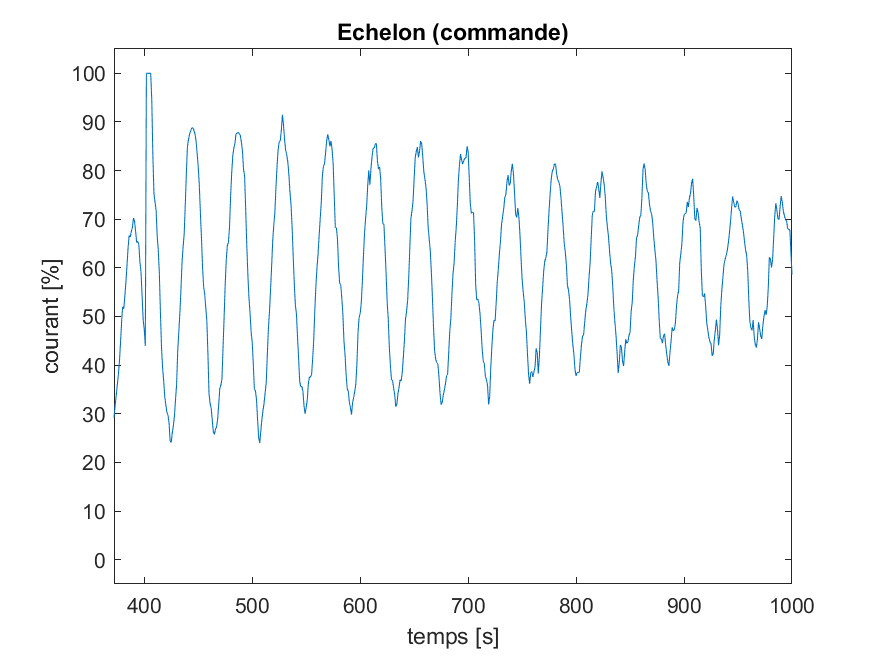
\includegraphics[width=\textwidth]{essais/s2e7-step-command}
        \end{subfigure}
        ~
        \begin{subfigure}[b]{0.37\textwidth}
            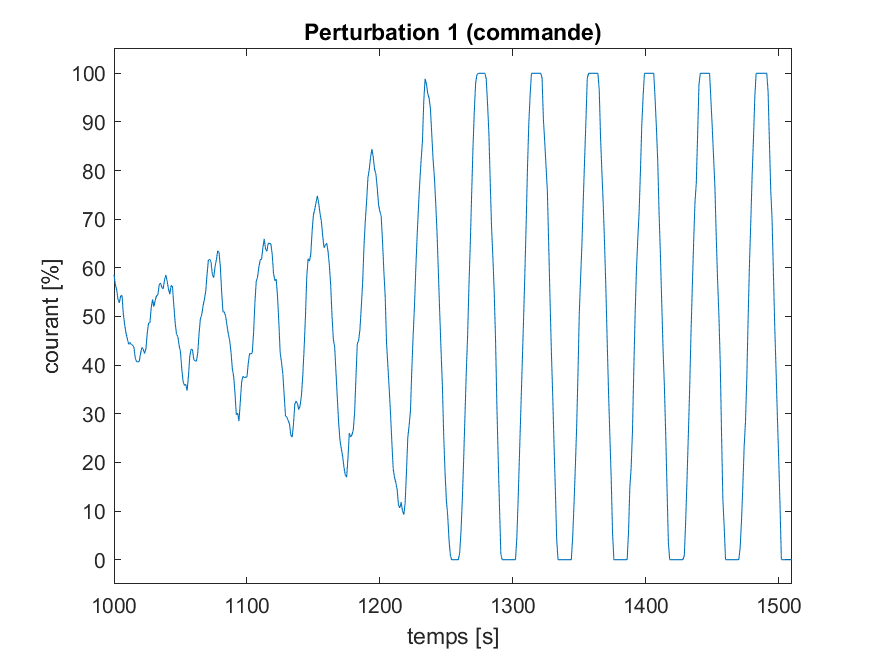
\includegraphics[width=\textwidth]{essais/s2e7-pert-up-command}
        \end{subfigure}
        ~
        \begin{subfigure}[b]{0.37\textwidth}
            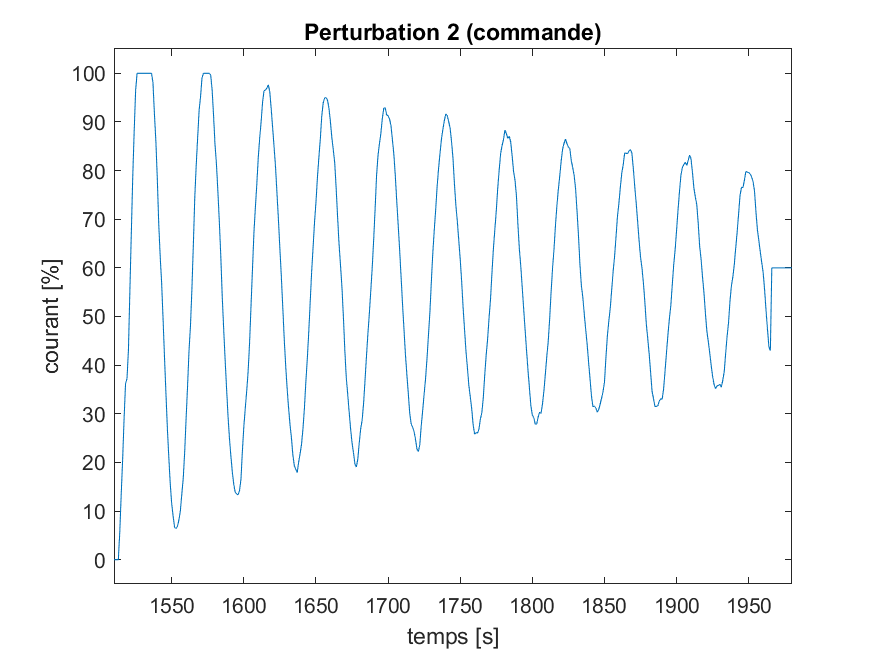
\includegraphics[width=\textwidth]{essais/s2e7-pert-down-command}
        \end{subfigure}
    }
    \caption{Graphes essai 7}
    \label{fig:essai-7}
\end{figure}

En augmentant trop le coefficient du terme dérivatif, le système frôle l'instabilité.
Les oscillations ont tendances à parfois diminuer, parfois augmenter. Dans le dernier
cas, le système s'emballe et est instable.

\fig{essais/bode-7}{0.5}{Diagramme de Bode}

\subsubsection{Essai 8 : $K_{p} = 8*K_{0}'$, $T_{i} = 10^{5}$ et $T_{d} = 10^{-3}$}
%Correspond au fichier s2e8

\begin{figure}[H]
    \centering
    % Line 1
    \makebox[\textwidth][c]{
        \begin{subfigure}[b]{0.37\textwidth}
            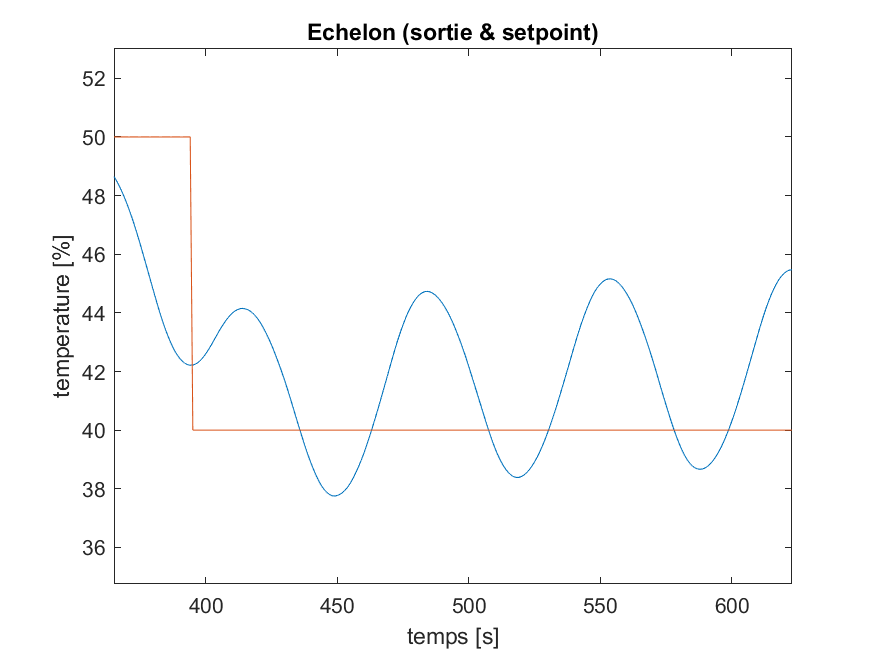
\includegraphics[width=\textwidth]{essais/s2e8-step-out}
        \end{subfigure}
    }
    % Line 2
    \makebox[\textwidth][c]{
        \begin{subfigure}[b]{0.37\textwidth}
            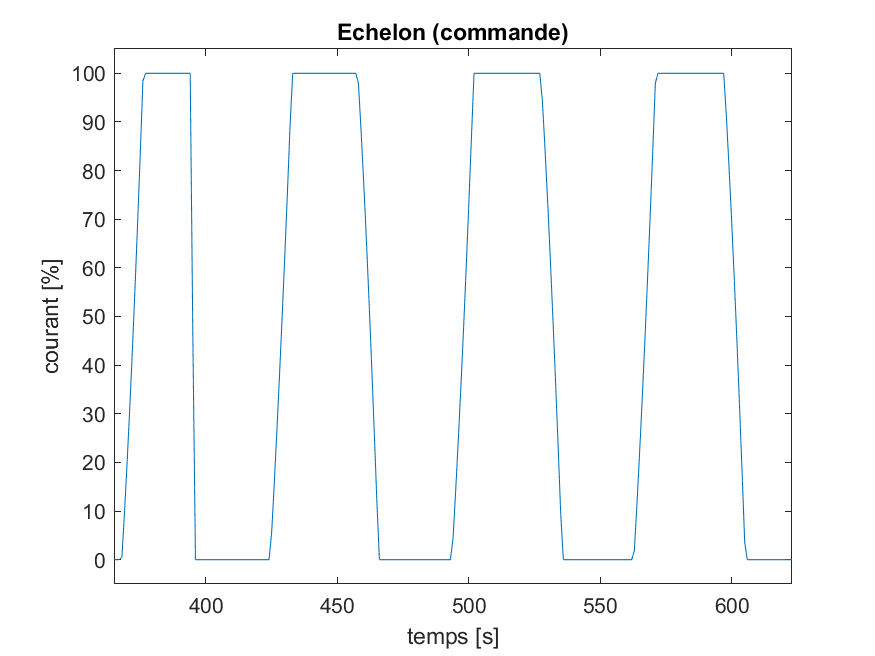
\includegraphics[width=\textwidth]{essais/s2e8-step-command}
        \end{subfigure}
    }
    \caption{Graphes essai 8}
    \label{fig:essai-8}
\end{figure}

Avec un terme proportionnel aussi important, le système part en instabilité.
On peut voir que le régulateur sature une fois dans un sens, une fois dans l'autre.
Comme les oscillations étaient grandes et n'allaient pas se résorber, nous
n'avons pas trouvé utiles d'appliquer les perturbations, car aucune conclusion
utile aurait pu en être déduite.

\fig{essais/bode-8}{0.5}{Diagramme de Bode}


\subsection{Régulateur optimisé}
La mesure de ces différents éssais nous a pris énormément de temps et nous n'avons donc pas
pu réaliser des essais afin d'obtenir un régulateur optimisé pendant la séance 2. Il sera 
fait pendant la séance 3 et donc traité dans la section \ref{opt-reg}.

